\chapter{Problem Formulation and Implementation}

The formulation of the guidance law is presented in this chapter, along with an overview of its implementation in numerical simulation.

\section{Problem Definition and Assumptions}
The objective of this project is to develop a feedback guidance law for transferring between two orbits around a planet in orbit around the Sun using a solar sail spacecraft.

Stated more formally, the problem is given as:

\fbox{\begin{minipage}{0.9\textwidth}
        \textbf{Planetocentric Solar Sail Feedback Guidance Problem}

        Consider a spacecraft propelled by an ideal flat solar sail with sail loading $\sigma$ and efficiency $\eta$ in an ideal 2-body orbit around a planet with gravitaional parameter $\mu$ (which itself orbits the Sun). Let be $P$ the radiation pressure of incident sunlight, which comes from a known direction $\hat{u}_i$.

        Given the instantaneous spacecraft state $\{p, f, g, h, k, L\}$ and target orbit described by the elements $\{\hat{p}, \hat{f}, \hat{g}, \hat{h}, \hat{k}\}$, determine an instantaneous spacecraft orientation in the LVLH frame (i.e. the sail normal $\hat{n}$, presented in the form of steering angles $\alpha$ and $\beta$) which ultimately brings the spacecraft to the target orbit.
    \end{minipage}}

The terms of this statement are elaborated in the proceeding subsections.

\subsection{Orbit and Environment}
\label{sec:orbit_environment}
The spacecraft is assumed to be orbiting a planet, possessing an instantaneous state expressed in modified equinoctial elements \{$p, f, g, h, k, L$\} (i.e an osculating orbit). The spacecraft is targeting an orbit described in modified equinoctial elements, as $\{\hat{p}, \hat{f}, \hat{g}, \hat{h}, \hat{k}\}$

The position of the spacecraft with respect to the planet is given by the vector $\vec{r}$, and the absolute velocity of the spacecraft is given by $\vec{v}$.



\textbf{Remark on Notation}: Mathematical notation for vectors follows the vectrix convention, as used in Ref. \cite{book:1487513}. Abstract vectorial quantities are written with the arrow above (e,g $\vec{u}$), and vectors expressed in a reference frame $\vec{\mathcal{F}}$ are written in boldface (e.g. $\boldsymbol{u}$). Unit vectors are given a special notation, written using a hat (e.g. $\hat{u}$).

\textbf{Reference Frames}

Two reference frames are used in this problem, defined in Table \ref{tab:frames_3d}, based on common convention. The frame $\mathcal{\vec{F}}_I$ has its origin at the center of the planet, and is taken to be inertial. The $\mathcal{\vec{F}}_{\text{LVLH}}$ is attached to the spacecraft, and its orientation is defined by the position vector of the spacecraft and the plane of the orbit.

\begin{table}[H]
    \centering
    \begin{tabular}{ccC{3cm}C{4cm}C{3cm}}
        \toprule
        Frame Name                         & Symbol                                   & $x$-direction                 & $y$-direction                                           & $z$-direction                            \\ \midrule
        Inertial                           & $\mathcal{\vec{F}}_I$                    & Points in direction of \aries & Perpendicular to $\hat{x}_I$ in equatorial plane        & $\hat{z}_I = \hat{x}_I \times \hat{y}_I$ \\
        LVLH                               & $\mathcal{\vec{F}}_{\text{LVLH}}$        & $\frac{\vec{r}}{||\vec{r}||}$ & $\frac{\vec{r} \times \vec{v} \times \vec{r}}{||\vec{r}
        \times \vec{v} \times \vec{r}||} $ & $\frac{\vec{r} \times \vec{v}}{||\vec{r}
        \times \vec{v}||} $                                                                                                                                                                                                \\
        \bottomrule
    \end{tabular}
    \caption{The frames involved, and their definitions.}
    \label{tab:frames_3d}
\end{table}

Quantities related to the guidance law are expressed in the LVLH frame, including steering command outputs. This choice of frame is motivated by past formulations of the \textit{Q-Law}, which are based on variational equations in the LVLH frame.

\textbf{Sun}

The Sun is located at a position $\vec{r}_{\astrosun}$ with respect to the planet, and hence the vector going from the Sun to the spacecraft is given by $\vec{r} - \vec{r}_{\astrosun}$. The direction of incident light is therefore given by $\hat{u} = -\frac{\vec{r} - \vec{r}_{\astrosun}}{||\vec{r} - \vec{r}_{\astrosun}||}$.

A diagram describing the elements of the problem discussed so far is shown in Figure \ref{fig:problem_setup}.
\begin{figure}[H]
    \centering
    \begin{subfigure}[t]{\textwidth}
\tdplotsetmaincoords{60}{30}
\begin{tikzpicture}[tdplot_main_coords,scale=1]
    \coordinate (O) at (0, 0, 0);
    \coordinate (SC) at ({9/sqrt(2)}, {9/sqrt(2)}, 0);
    \coordinate (SUN) at (0, 6, 2);
    % Orbit 1
    \begin{scope}[plane x={({1/sqrt(2)}, {1/sqrt(2)}, 0)}, plane y={(-0.5, 0.5, {1/sqrt(2)})}, canvas is plane]
    % Grid
    \begin{scope}[densely dotted, green!50!black]
    \draw (-1, 0, 0) -- (9, 0, 0);
    \draw (0, -1.8, 0) -- (0, 1.8, 0);
    \end{scope}
    \draw[green!50!black, thick, fill=green!50!black, fill opacity=0.2] (4, 0, 0) ellipse (5cm and 3cm);
    \draw (9, -0.5) node[below right, green!50!black, text width=4cm]{Instantaneous Spacecraft State $\{p, f, g, h, k, L\}$};
    \end{scope}
    % Orbit 2
    \begin{scope}[plane x={(1, 0, 0)}, plane y={(0, 1, 0)}, canvas is plane]
    % Grid
    \begin{scope}[densely dotted, red!50!black]
    \draw (-2, 0, 0) -- (8, 0, 0);
    \draw (0, -3, 0) -- (0, 3, 0);
    \end{scope}
    \draw[red!50!black, thick, fill=red!50!black, fill opacity=0.2] (3, 0, 0) ellipse (5cm and 4cm);
    \draw (8, 0) node[below right, red!50!black, text width=5cm]{Target Orbit $\{\hat{p}, \hat{f}, \hat{g}, \hat{h}, \hat{k}\}$};
    \end{scope}
    \draw[dashdotted, cyan!50!black] (SUN) -- (SC);
    % Sun
    \fill[color=yellow] (SUN) 
    circle(0.5cm);
    % SC
    \fill[black] (SC) circle(0.1cm);
    % to SC and Sun
    \begin{scope}[-latex, orange, very thick]
    \draw (O) -- (SC) node[pos=0.8, below right]{$\vec{r}$};
    \draw (O) -- (SUN) node[pos=0.7, above left]{$\vec{r}_{\astrosun}$};
    \draw[cyan!50!black] (SUN) -- ($(SUN)!0.2!(SC)$) node[pos=0.7, above right]{$\vec{u}_{i}$};
    \end{scope}
    % Earth
    \fill[earthblue] (0, 0) circle(0.5cm);
    % Axes
    \begin{scope}[-latex, thick]
        \draw (O) -- ++ (2,0,0) node[below]{$\hat{x}_{I}$};
        \draw (O) -- ++ (0,2,0) node[right]{$\hat{y}_{I}$};
        \draw (O) -- ++ (0,0,2) node[right]{$\hat{z}_{I}$};
        \draw (SC) -- ++ ({2/sqrt(2)},{2/sqrt(2)},0) node[right]{$\hat{x}_{\text{LVLH}}$};
        \draw (SC) -- ++ (-1,1,{2/sqrt(2)}) node[right]{$\hat{y}_{\text{LVLH}}$};
        \draw (SC) -- ++ (1,-1,{2/sqrt(2)}) node[above right]{$\hat{z}_{\text{LVLH}}$};
    \end{scope}
\end{tikzpicture}
\caption{Spatial setup of problem, primary view.}
\label{fig:problem_setup:view1}
\end{subfigure}
    \begin{subfigure}[t]{\textwidth}
\tdplotsetmaincoords{80}{110}
\begin{tikzpicture}[tdplot_main_coords,scale=1]
    \coordinate (O) at (0, 0, 0);
    \coordinate (SC) at ({9/sqrt(2)}, {9/sqrt(2)}, 0);
    \coordinate (SUN) at (0, 6, 2);
    % Orbit 1
    \begin{scope}[plane x={({1/sqrt(2)}, {1/sqrt(2)}, 0)}, plane y={(-0.5, 0.5, {1/sqrt(2)})}, canvas is plane]
    % Grid
    \begin{scope}[densely dotted, green!50!black]
    \draw (-1, 0, 0) -- (9, 0, 0);
    \draw (0, -1.8, 0) -- (0, 1.8, 0);
    \end{scope}
    \draw[green!50!black, thick,  fill=green!50!black, fill opacity=0.2] (4, 0, 0) ellipse (5cm and 3cm);
    \end{scope}
    % Orbit 2
    \begin{scope}[plane x={(1, 0, 0)}, plane y={(0, 1, 0)}, canvas is plane]
    % Grid
    \begin{scope}[densely dotted, red!50!black]
    \draw (-2, 0, 0) -- (8, 0, 0);
    \draw (0, -3, 0) -- (0, 3, 0);
    \end{scope}
    \draw[red!50!black, thick, fill=red!50!black, fill opacity=0.2] (3, 0, 0) ellipse (5cm and 4cm);
    \end{scope}
    \draw[dashdotted, cyan!50!black] (SUN) -- (SC);
    % Sun
    \fill[color=yellow] (SUN) 
    circle(0.5cm);
    % SC
    \fill[black] (SC) circle(0.1cm);
    % to SC and Sun
    \begin{scope}[-latex, orange, very thick]
    \draw (O) -- (SC) node[pos=0.7, below left]{\(\vec{r}\)};
    \draw (O) -- (SUN) node[pos=0.9, above left]{\(\vec{r}_{\astrosun}\)};
    \draw[cyan!50!black] (SUN) -- ($(SUN)!0.2!(SC)$) node[pos=, below right]{\(\vec{u}_{i}\)};
    \end{scope}
    % Earth
    \fill[earthblue] (0, 0) circle(0.5cm);
    % Axes
    \begin{scope}[-latex, thick]
        \draw (O) -- ++ (2,0,0) node[below]{\(\hat{x}_{I}\)};
        \draw (O) -- ++ (0,2,0) node[right]{\(\hat{y}_{I}\)};
        \draw (O) -- ++ (0,0,2) node[right]{\(\hat{z}_{I}\)};
        \draw (SC) -- ++ ({2/sqrt(2)},{2/sqrt(2)},0) node[right]{\(\hat{x}_{\text{LVLH}}\)};
        \draw (SC) -- ++ (-1,1,{2/sqrt(2)}) node[right]{\(\hat{y}_{\text{LVLH}}\)};
        \draw (SC) -- ++ (1,-1,{2/sqrt(2)}) node[above right]{\(\hat{z}_{\text{LVLH}}\)};
    \end{scope}
\end{tikzpicture}
\caption{Spatial setup of problem, alternate view.}
\label{fig:problem_setup:view2}
\end{subfigure}
    \caption{Diagram of key elements of the problem (multiple views for clarity). The planet is represented by the blue circle, the Sun by the yellow circle, and the spacecraft by the black dot.}
    \label{fig:problem_setup}
\end{figure}

% another diagram for steering convention

\subsection{Spacecraft Orientation Convention}
The output of the guidance law is a spacecraft orientation in the LVLH frame. That is, the guidance law expresses the unit vector $\hat{n}$ in terms of the output steering angles $\alpha$ and $\beta$.

The convention used in this project follows Refs. \cite{petropoulos2004low, vargaperez2016, sanjeev2023}, and is depicted in Figure \ref{fig:orientation_convention}.

\begin{figure}[H]
    \centering
    \tdplotsetmaincoords{65}{140}
    \begin{tikzpicture}[tdplot_main_coords,scale=1]
        \coordinate (O) at (0,0,0);
        \coordinate (B) at (-2,0,0);
        \coordinate (N) at (4, 2, 4.6);
        \coordinate (NP) at (4, 2, 0);
        % R Arrow
        \draw[dashed, orange, thick, -latex] (B) -- (O) node[pos=0.1, above]{\(\vec{r}\)};
        % horizon line
        \draw[densely dotted, black!50] (O) ++(1, -4, 0) -- ++(-2, 8, 0);
        \begin{scope}[-latex, thick]
            \draw (O) -- ++ (3,0,0) node[left]{\(\hat{x}_{\text{LVLH}}\)};
            \draw (O) -- ++ (0,3,0) coordinate (Y) node[below]{\(\hat{y}_{\text{LVLH}}\)};
            \draw (O) -- ++ (0,0,3) node[above right]{\(\hat{z}_{\text{LVLH}}\)};
        \end{scope}
        % Arc
        \draw[densely dashdotted, green!70!black, thick] (O) arc (10:50:7) (O) arc(10:-30:7);
        % Stuff
        \draw[very thick, -latex, purple] (O) -- (N) node[left]{\(\hat{n}\) (Direction of \(\vec{F}\))};
        \draw[purple] (O) -- (NP) -- (N);
        % Angles
        \begin{scope}[canvas is xy plane at z=0]
            \draw pic["\(\alpha\)", draw=purple, text=purple, latex-|, thick, angle eccentricity=1.3, angle radius=1.2cm,transform shape, pic text options={transform shape=false}] {angle=NP--O--Y};
        \end{scope}
        \draw pic["\(\beta\)", draw=purple, text=purple, latex-|, thick, angle eccentricity=1.4, angle radius=1cm,transform shape] {angle=N--O--NP};
    \end{tikzpicture}
    \caption{Thrust angle orientation convention. Note that generally, \(\alpha = 0\) does NOT correspond to the direction of the velocity vector of the spacecraft, as \(\vec{\mathcal{F}}_{\text{LVLH}}\) is aligned with \(\vec{r}\) and \(\vec{r} \times \vec{v}\). The dashed grey line represents the tangent line to the orbit, which is generally not aligned with \(\hat{y}_{\text{LVLH}}\).}
    \label{fig:orientation_convention}
\end{figure}
$\alpha$ is a clockwise steering angle from the $y$-axis in the $xy$ LVLH plane, and $\beta$ is a steering angle towards the $+z$ axis.

That is to say, the direction vector of the spacecraft is given by:
\begin{equation}
    \hat{n}(\alpha, \beta) = \mathcal{\vec{F}}_{\text{LVLH}}^T
    \begin{bmatrix}
        \cos \beta \sin \alpha \\
        \cos \beta \cos \alpha \\
        \sin \beta
    \end{bmatrix}
    \label{eq:alpha_beta_n}
\end{equation}


\subsection{Dynamics}
\textbf{Sail Thrust}

Dynamics for an idealized flat solar sail are presented and used in the implementation of numerical simulations.

For a solar sail pointing in the direction $\hat{n}$ and for incident light in the direction $\hat{u}_i$, the acceleration imparted on the sail is given by:
\begin{equation}
    \vec{F} = \frac{2 P \eta}{\sigma}(\hat{u}_i \cdot \hat{n})^2 \mathrm{sign}(\hat{u}_i \cdot \hat{n}) \hat{n}
    \ [\unit{m\ s^{-2}}] \label{eq:solar_force}
\end{equation}

Where $P = \qty{9.12e-6}{N\ m^{-2}}$ is the value of solar radiation pressure at a distance of 1 AU. The quantity $\sigma = \frac{m}{A}$ [\unit{kg\ m^{-2}}] referred to as \textit{sail loading} is the mass of the spacecraft divided by the sail area, and is conventionally used to parameterize sail performance. A dimensionless efficiency factor $\eta$ represents ``how reflective'' the material of the sail is, relative to a perfect reflector. The leading coefficient of 2 results from force imparted both by incident and reflected photons.

\textbf{Variational Equations of Motion}

The equations of motion of the spacecraft are given by (\ref{eq:equinoctial_eom_3d}) below.
\begin{equation}
    \diff{}{t}
    {
        \renewcommand*{\arraystretch}{1.2}
        \begin{bmatrix}
            p \\f\\g\\h\\k\\L
        \end{bmatrix}}
    =
    \frac{1}{q}\sqrt{\frac{p}{\mu}}
    {
        \renewcommand*{\arraystretch}{1.2}
        \begin{bmatrix}
            0        & 2p               & 0                                 \\
            q\sin L  & (q+1) \cos L + f & -g(h \sin L - k \cos L)           \\
            -q\cos L & (q+1) \sin L + g & f(h \sin L - k \cos L)            \\
            0        & 0                & \tfrac{\cos L}{2} (1 + h^2 + k^2) \\
            0        & 0                & \tfrac{\sin L}{2} (1 + h^2 + k^2) \\
            0        & 0                & h \sin L - k \cos L
        \end{bmatrix}}
    {\begin{bmatrix}
            F_r      \\
            F_\theta \\
            F_n
        \end{bmatrix}}
    +
    {
    \renewcommand*{\arraystretch}{1.2}
    \begin{bmatrix}
        0 \\0\\0\\0\\0\\
        \frac{q^2 \sqrt{\mu p}}{p^2}
    \end{bmatrix}} \label{eq:equinoctial_eom_3d}
\end{equation}
\begin{align*}
    \text{with} \ \ q & \equiv 1 + f\cos L + g\sin L
    \intertext{$F_r$, $F_\theta$, $F_n$ correspond to perturbing accelerations on the spacecraft expressed in the LVLH frame corresponding to the radial, tangential, and normal directions respectively. That is:}
    \vec{F}           & =
    \mathcal{\vec{F}}_{\mathrm{LVLH}}^T
    \begin{bmatrix}
        F_r \\F_\theta\\F_n
    \end{bmatrix}
\end{align*}





\subsection{Motion of the Sun}
The sun is assumed to be \qty{1.5e8}{m} from the center of the coordinate system, at an angle varying by $2\pi$ in 1 year ($\tau = \qty{365.25}{d} = \qty{31557600}{s}$).

That is,
\begin{equation}
    \vec{r}_{\astrosun}(t) =
    \num{1.5e8}
    \
    \mathcal{\vec{F}}_I^T
    \begin{bmatrix}
        \cos(\lambda_{\astrosun})                   \\
        \sin(\lambda_{\astrosun}) \cos(\varepsilon) \\
        \sin(\lambda_{\astrosun}) \sin(\varepsilon)
    \end{bmatrix}
    \unit{m}
    \label{eq:sun_position_3d}
\end{equation}
Where $\lambda_{\astrosun} = \frac{2 \pi}{\tau} t$, with $t=0$ corresponding to the vernal equinox, and $\varepsilon = \ang{23.439}$ is the obliquity of the ecliptic.

This is obviously not reflective of Earth's elliptical orbit around the Sun, but it is assumed to be adequate as a starting point.

In this analysis, the position of the Sun is considered to be \textbf{quasi-static}, that is, $\dot{\lambda}_{\astrosun} = 0$, since the motion of the Sun occurs on a timescale much longer than the period of an orbit.

\section{Methodology}
The guidance law is implemented in a
two-stage architecture, depicted in Figure \ref{fig:algorithm_diagram} below. The guidance law occupies the left half of the diagram (blocks in blue and green), while the rest of the dynamics are shown in the purple blocks on the right.

\begin{figure}[H]
    \centering
    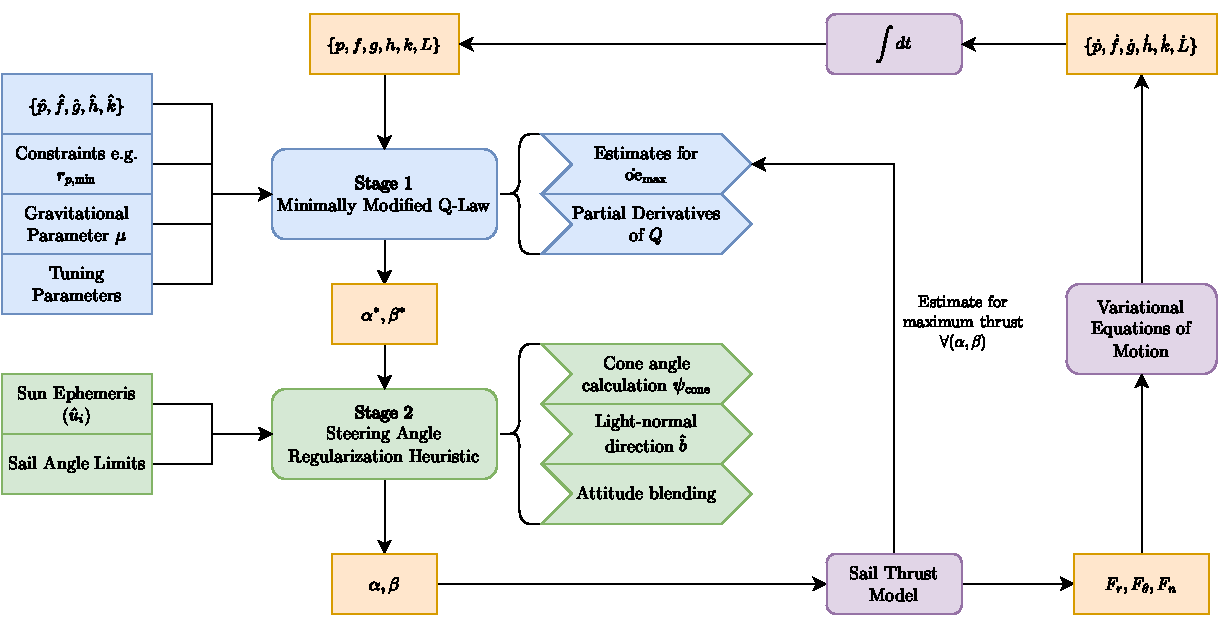
\includegraphics[width=\textwidth]{figures/compute_topology.drawio.pdf}
    \caption{Architecture of the guidance law, along with the dynamics of the spacecraft.}
    \label{fig:algorithm_diagram}
\end{figure}

The key idea is to consider all solar sail-related elements (direction of incident light, restrictions on orientation) independently of the formulation for the ``idealized'' steering angles. The first stage of the guidance law treats the solar sail as if it were a regular low-thrust spacecraft capable of producing an acceleration $F_{\max}$ at constant thrust. From this, it generates idealized angles $\alpha^*, \beta^*$, which are then regularized by the second stage to make them feasible for a solar sail to use.

Rather than try to rework the \textit{Q-Law}, the heuristic attached to the original guidance law transforms the solar sail guidance problem into a more conventional low-thrust guidance problem with modified dynamics. That is, the steering angle regularization block can be thought of as being part of the dynamics, with the \textit{Q-Law} operating as if it were controlling a regular low-thrust spacecraft.

\section{Formulation of Minimally Modified Q-Law}
The minimally modified \textit{Q-Law} is derived in this section, along with a computational procedure for assembling the steering angle outputs.

\subsection{Control-Lyapunov Function}
The minimally modified \textit{Q-Law} is structured very similarly to previous works (Refs. \cite{petropoulos2004low, vargaperez2016, sanjeev2023}), following a control-Lyapunov function $Q$, which is then differentiated in terms of steering angles $\alpha, \beta$ to determine the direction maximizing $-\dot{Q}$.

The control-Lyapunov function is given below in Equation \ref{eq:Q_func}.
\begin{align}
    Q        & = (1+W_P P) \sum_{\moe} W_{\moe} S_{\moe} \left(\frac{\moe - \hat{\moe}}{\dot{\moe}_{\maxrocall}} \right)^2 \ \, \moe \in \{p, f, g, h, k\} \label{eq:Q_func} \\
    S_{\moe} & = \begin{cases}
                     \frac{1}{R_e} & \moe = p         \\
                     1             & \text{Otherwise} \\
                 \end{cases} \nonumber                                                                                                                            \\
    P        & = \exp\left[\gamma \left( 1 - \frac{r_p}{r_{p, \text{min}}} \right) \right] \nonumber                                                                         \\
    a        & = \frac{p}{1-e^2} \nonumber                                                                                                                                   \\
    r_{p}    & = a (1-e) = p\frac{(1-e)}{(1+e)(1-e)} = \frac{p}{1+\sqrt{f^2 + g^2}} \nonumber
\end{align}
with $\dot{\moe}_{\maxrocall}$ being taken to mean the maximum achieveable rate of change in that orbital element for any value of steering angles $(\alpha, \beta)$ and true longitude $L$.

The only variables in $Q$ are $\moe \in \{p, f, g, h, k\}$, and therefore $Q$ can be written as a sum of derivatives using the chain rule:
\begin{align*}
    \dot{Q} & = \sum_{\moe} \diffp{Q}{{\moe}} \dot{\moe}
\end{align*}
Note that Equation \ref{eq:equinoctial_eom_3d} in fact gives $\dot{\moe}$ as a function of $F_r, F_\theta, F_n$. The idea then is to link $\dot{Q}$ to the thrust model for the solar sail, without being overly specific. The key assumption taken for deriving the \textit{Q-Law} portion of the guidance law is to \textbf{assume that the solar sail always produces its maximum possible thrust in any direction} (i.e. Figure \ref{fig:thrust_curve}). Hence, Equation \ref{eq:max_accel_assumption} is taken to be true for the purposes of deriving ideal steering angles.
\begin{equation}
    \begin{bmatrix}
        F_r      \\
        F_\theta \\
        F_n
    \end{bmatrix} =
    \frac{2P\eta}{\sigma}
    \begin{bmatrix}
        \cos \beta \sin \alpha \\
        \cos \beta \cos \alpha \\
        \sin \beta
    \end{bmatrix}
    \equiv
    F_{\max}
    \begin{bmatrix}
        \cos \beta \sin \alpha \\
        \cos \beta \cos \alpha \\
        \sin \beta
    \end{bmatrix}
    \label{eq:max_accel_assumption}
\end{equation}
Keeping the relationship simple using only $F_{\max}$ allows for a very general application of the guidance law to a broad range of spacecraft configurations.

\begin{figure}
    \centering
    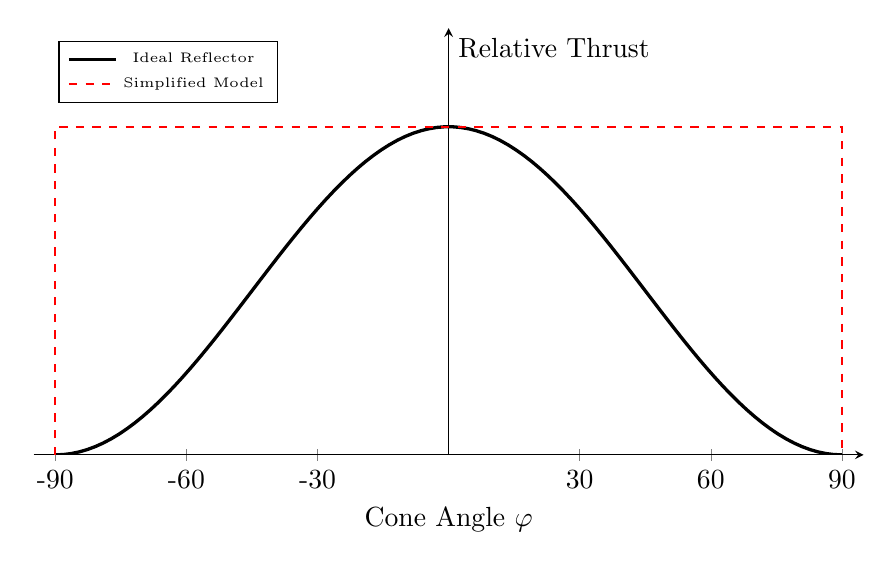
\begin{tikzpicture}
        \begin{axis}[
                axis lines = middle,
                ymax = 1.3,
                xmin = -95,
                xmax = 95,
                xlabel ={Cone Angle $\varphi$},
                xlabel near ticks,
                ylabel = {Relative Thrust},
                xtick={-90, -60, -30, 0, 30, 60, 90},
                xticklabels={\ang{-90}, \ang{-60}, \ang{-30}, \ang{0}, \ang{30}, \ang{60}, \ang{90}},
                legend pos=north west,
                ytick=\empty,
                height=7cm,
                width=\textwidth
            ]
            \addplot [
                domain=-90:90,
                samples=100,
                color=black,
                very thick
            ]
            {cos(x)^2};
            \addlegendentry{\tiny Ideal Reflector}
            \addplot+[thick,mark=none, dashed,const plot]
            coordinates
                {(-90,0) (-90,1) (90, 1) (90, 0)};
            \addlegendentry{\tiny Simplified Model}
        \end{axis}
    \end{tikzpicture}
    \caption{A significant assumption being made for the Q-Law portion of the guidance law is to remove the direction-dependence on produced thrust.}
    \label{fig:thrust_curve}
\end{figure}

\subsection{Ideal Steering Angles}
By simultaneously considering Equations \ref{eq:equinoctial_eom_3d} and \ref{eq:max_accel_assumption}, $\dot{\moe}$ becomes a function of $\alpha$ and $\beta$.

$\dot{Q}$ can therefore be expressed in a form based on steering angles, shown below:
\begin{align}
    \dot{Q}  & = D_1 \cos \beta \sin \alpha + D_2 \cos \beta \cos \alpha + D_3 \sin \beta \label{eq:q_dot_angles_form} \\
    \intertext{For some $D_1$, $D_2$, $D_3$ based on other variables/parameters. Finding the stationary point of $\dot{Q}$ with respect to $(\alpha, \beta)$ gives:}
    \alpha^* & = \mathrm{atan2}\left(-D_1, -D_2\right) \label{eq:alpha_star}                                           \\
    \beta^*  & = \mathrm{atan2}\left(-D_3, \sqrt{D_1^2 + D_2^2}\right) \label{eq:beta_star}
\end{align}
which maximizes $-\dot{Q}$. This form is obtained from Ref. \cite{vargaperez2016}, where the definition of $D_1$ and $D_2$ are swapped compared to this project. The reasoning behind the ordering here is such that $D_1, D_2, D_3$ line up with $F_r, F_\theta, F_n$.

\subsection{Assembling the Guidance Output}
The remaining piece consists of deriving expressions for all of the terms in $Q$ and $\dot{Q}$ and assembling them to produce optimal steering angles.

\textbf{Expressions for $\dot{\moe}_{\maxrocall}$}

$\dot{f}_{\maxrocall}$ and $\dot{g}_{\maxrocall}$ are taken as approximate analytical forms, first developed by Ref. \cite{vargaperez2016}. The other 3 orbital elements have exact analytical expressions for maximum rate of change, obtained by manipulating Equation \ref{eq:equinoctial_eom_3d}.
\begin{align*}
    \dot{p}_{\maxrocall} & = \frac{2p}{q} \sqrt{\frac{p}{\mu}} F_{\max}                                   \\
    \dot{f}_{\maxrocall} & \approx 2F_{\max} \sqrt{\frac{p}{\mu}}                                       &
    \dot{g}_{\maxrocall} & \approx 2F_{\max} \sqrt{\frac{p}{\mu}}                                         \\
    \dot{h}_{\maxrocall} & = \tfrac{1}{2}F_{\max} \sqrt{\frac{p}{\mu}} \frac{1+h^2+k^2}{\sqrt{1-g^2}+f} &
    \dot{k}_{\maxrocall} & = \tfrac{1}{2}F_{\max} \sqrt{\frac{p}{\mu}}\frac{1+h^2+k^2}{\sqrt{1-f^2}+g}
\end{align*}

\textbf{Partials of $Q$}

Each partial derivative of $Q$ can be written as:
\begin{equation*}
    \diffp{Q}{{\moe}} = W_{\moe} S_{\moe} \left[ W_P\diffp{P}{{\moe}}\left(\frac{\moe - \hat{\moe}}{\dot{\moe}_{\maxrocall}} \right)^2 + 2 (1+W_P P) \left(\frac{\moe - \hat{\moe}}{\dot{\moe}_{\maxrocall}} \right) \right] \ \, \moe \in \{p, f, g, h, k\}
\end{equation*}
The final forms of $D_1, D_2, D_3$ can now be computed from this, with a few shorthands introduced for convenience:
\begin{align*}
    \boldsymbol{\Xi}_E & = \begin{bmatrix}
                               2  \left(\frac{\moe - \hat{\moe}}{\dot{\moe}_{\maxrocall}} \right)
                           \end{bmatrix}_{\moe \in \{p, f, g, h, k\}} \in \mathbb{R}^5                                                 \\
    \boldsymbol{\Xi}_P & = \begin{bmatrix}
                               \diffp{P}{{\moe}}\left(\frac{\moe - \hat{\moe}}{\dot{\moe}_{\maxrocall}} \right)^2
                           \end{bmatrix}_{\moe \in \{p, f, g, h, k\}} \in \mathbb{R}^5 \\
    W                  & = \mathrm{diag} \left(\begin{bmatrix}
                                                   W_{\moe}
                                               \end{bmatrix}_{\moe \in \{p, f, g, h, k\}} \right) \in \mathbb{R}^{5 \times 5}                                                                                              \\
    S                  & = \mathrm{diag} \left(\begin{bmatrix}
                                                   S_{\moe}
                                               \end{bmatrix}_{\moe \in \{p, f, g, h, k\}}\right)  \in \mathbb{R}^{5 \times 5}                                                                                              \\
    A                  & =
    \begin{bmatrix}
        0        & 2p               & 0                                 \\
        q\sin L  & (q+1) \cos L + f & -g(h \sin L - k \cos L)           \\
        -q\cos L & (q+1) \sin L + g & f(h \sin L - k \cos L)            \\
        0        & 0                & \tfrac{\cos L}{2} (1 + h^2 + k^2) \\
        0        & 0                & \tfrac{\sin L}{2} (1 + h^2 + k^2)
    \end{bmatrix} \in \mathbb{R}^{5 \times 3}
    \intertext{\hfill ($q$ is defined in Equation \ref{eq:equinoctial_eom_3d}).}
    \boldsymbol{D}     & = \begin{bmatrix}
                               D_1 \\D_2\\D_3
                           \end{bmatrix} \in \mathbb{R}^3
\end{align*}
Combining everything together gives:
\begin{equation}
    \boldsymbol{D} = \begin{bmatrix}
        D_1 \\D_2\\D_3
    \end{bmatrix} = A^T W S \left(W_P \boldsymbol{\Xi}_P + (1 + W_P P) \boldsymbol{\Xi}_E \right)
\end{equation}

Combined with Equations \ref{eq:alpha_star} and \ref{eq:beta_star}, this gives a computational procedure for the ideal steering angles.

Note that $\diffp{P}{{\moe}}$ is calculated using symbolic algebra, and the expressions are omitted here because they are very ugly. It should be noted that $\diffp{P}{{\moe}}$ is nonzero only for $\moe \in \{p, f, g\}$.

\section{Beyond the Q-Law}
A solar-sail-agnostic formulation of the Q-Law is insufficient as a guidance law. There are two notable problem cases which arise from

\begin{figure}[H]
    \centering
    \begin{subfigure}[b]{0.45\textwidth}
        \centering
        \tdplotsetmaincoords{85}{20}
        \begin{tikzpicture}[tdplot_main_coords,scale=0.5]
            \coordinate (O) at (0,0,0);
            \coordinate (NS2) at ({5/sqrt(2)},{5/sqrt(2)},-2);
            \coordinate (NS3) at ({-5/sqrt(2)},{-5/sqrt(2)},2);
            \coordinate (T) at (0,0,5);
            % Cone stuff
            \draw[cyan!50!black, dashdotted] (O) -- (T);
            \draw[cyan!50!black, -latex] (O) ++(0,0,-2) -- (O) node[midway, left]{$\hat{u}_i$};
            % Adaptation
            \draw[-latex, dashed] (O) -- (NS2) node[right]{$\hat{n}^*$};
            \begin{scope}[canvas is xy plane at z = 0]
                \filldraw[draw=black!60, fill=black!50, fill opacity=.3] (0, 0) circle (3cm);
            \end{scope}
            \draw[-latex, green!70!black, thick] (O) -- (NS3) node[above]{\scriptsize Thrust};
        \end{tikzpicture}
        \caption{$\varphi > \ang{90}$ - Unstable}
        \label{fig:degencase_1}
    \end{subfigure}
    \begin{subfigure}[b]{0.45\textwidth}
        \centering
        \tdplotsetmaincoords{85}{20}
        \begin{tikzpicture}[tdplot_main_coords,scale=0.5]
            \coordinate (O) at (0,0,0);
            \coordinate (NS2) at ({5/sqrt(2)},{5/sqrt(2)},0.2);
            \coordinate (NS3) at ({1/sqrt(2)},{1/sqrt(2)},0.04);
            \coordinate (T) at (0,0,5);
            % Cone stuff
            \draw[cyan!50!black, dashdotted] (O) -- (T);
            \draw[cyan!50!black, -latex] (O) ++(0,0,-2) -- (O) node[midway, left]{$\hat{u}_i$};
            \begin{scope}[canvas is xy plane at z = 0]
                \filldraw[draw=black!60, fill=black!50, fill opacity=.3] (0, 0) circle (3cm);
            \end{scope}
            % Adaptation
            \draw[-latex, dashed] (O) -- (NS2) node[right]{$\hat{n}^*$};
            \draw[-latex, green!70!black, thick] (O) -- (NS3) node[above]{\scriptsize Thrust};
        \end{tikzpicture}
        \caption{$\varphi \approx \ang{90}$ - No Progress}
        \label{fig:degencase_2}
    \end{subfigure}
    \caption{Problematic cases associated with a solar-sail-agnostic guidance law.}
    \label{fig:degencases}
\end{figure}

\section{Steering Angle Regularization Heuristic}
The steering angle heuristic is formulated in this section, beginning from the conceptual motivation of the idea.

\subsection{Concept}
If the cone angle produced by the ideal steering angles from the first stage is outside the achievable range of the solar sail, there are two options:
\begin{enumerate}
    \setlength{\parskip}{2pt}
    \item \textbf{Feather the sail}: Orient the solar sail (normal) at exactly \ang{90} relative to the incident sunlight to produce zero thrust.
    \item \textbf{Make a Compromise}: Find the ``closest'' valid sail orientation, subject to the cone angle restriction. (This notion of ``closeness'' is elaborated upon in the formulation).
\end{enumerate}

Feathering the sail is useful for situations where the cone angle suggested by the first stage exceeds \ang{90} (i.e. the sail cannot produce thrust in that direction). This prevents the spacecraft from regressing \textbf{away} from its target orbit.

The latter option is particularly helpful even in the case of an ideal flat solar sail, where the first stage of the guidance law could produce a set of steering angles resulting in a cone angle very close to \ang{90}. The thrust produced in such a situation would be extremely small, and result in less progress being made compared to if the guidance law accepted a thrust direction which does not point exactly towards the local optimum. By accepting a non-ideal direction, the spacecraft can still make progress towards its goal.

\subsection{Formulation}
The ideal steering angles $\alpha^*, \beta^*$ are used to compute an idealized cone angle.
\begin{equation}
    \varphi^* = \arccos(\hat{u}_i \cdot \hat{n}^*)
    \label{eq:cone_star}
\end{equation}
where $\hat{n}^* = \hat{n}(\alpha^*, \beta^*)$ can be computed using (\ref{eq:alpha_beta_n}) and $\hat{u}_i = -\frac{\vec{r}_{\astrosun}}{||\vec{r}_{\astrosun}||}$. Both vectors are expressed in the same frame for computational procedures (e.g. the LVLH frame).

$\varphi^*$ is compared between cone angle thresholds:
\begin{enumerate}
    \item \textbf{Feathering Threshold}: $\varphi = \ang{90}$
    \item \textbf{Degraded Operation Threshold}: $\varphi = \kappa$
\end{enumerate}

Consider a vector $\hat{b}$ which is normal to both $\hat{u}_i$ and $\hat{n}^*$. For example, $\hat{b} = \hat{u}_i \times (\hat{n}^* \times \hat{u}_i)$.

The resulting sail normal $\hat{n}$ is then calculated as:
\begin{equation}
    \hat{n} = \begin{cases}
        \hat{n}^*                                       & \cos \varphi^* > \cos \kappa          \\
        \cos \kappa \ \hat{u}_i + \sin \kappa \ \hat{b} & \cos \varphi^* \in  [ 0, \cos \kappa] \\
        \hat{b}                                         & \cos \varphi^* < 0
    \end{cases}
    \label{eq:ndf_law}
\end{equation}

The 3 cases in Equation \ref{eq:ndf_law} correspond to \textbf{nominal, degraded, and feathered} operation.

\begin{figure}[H]
    \centering
    \tdplotsetmaincoords{85}{45}
    \begin{tikzpicture}[tdplot_main_coords,scale=1]
        \coordinate (O) at (0,0,0);
        \coordinate (KD) at ({2/sqrt(2)},{2/sqrt(2)},3);
        \coordinate (NS) at ({2.5/sqrt(2)},{2.5/sqrt(2)},2.5);
        \coordinate (KF) at ({3/sqrt(2)},{3/sqrt(2)},0);
        \coordinate (T) at (0,0,7);
        % BG
        \begin{scope}[plane x={({1/sqrt(2)}, {1/sqrt(2)}, 0)}, plane y={(0, 0, 1)}, canvas is plane]
            \fill[green!10!white] (O) -- (90:6) arc(90:56.31:6) node[midway, above=4pt, text=green!70!black]{\footnotesize{Unmodified}} -- cycle;
            \fill[yellow!10!white] (O) -- (56.31:6) arc(56.31:0:6) node[midway, above right=4pt, text=yellow!70!black]{\footnotesize{Projected}} -- cycle;
            \fill[black!10] (O) -- (0:6) arc(0:-18:6) node[midway, right, text=black!70]{\footnotesize{Feathered}} -| (O) -- cycle;
        \end{scope}
        % Cone stuff
        \coneback[draw=yellow!70!black, fill=yellow!40!white, fill opacity=.6]{3}{2}{0}
        \begin{scope}[thick, cyan!50!black]
            \draw[dashdotted] (O) -- (T);
            \draw[-latex] (O) ++(0,0,-2) -- (O) node[midway, left]{Incident Light $\hat{u}_i$};
        \end{scope}
        \conefront[draw=yellow!70!black, fill=yellow!40!white, fill opacity=.6]{3}{2}{0}
        \begin{scope}[canvas is xy plane at z = 0]
            \filldraw[draw=black!60, fill=black!50, fill opacity=.3] (0, 0) circle (3cm);
        \end{scope}
        % Annotations of thrust cone and limit plane
        \draw[yellow!70!black] (O) ++(-1, 0, 3.5) node[left] {Thrust Cone};
        \draw[black!60] (O) ++(-1, 0, 0.75) node[left] {Limit Plane};
        % Angles
        \draw pic["$\kappa$", draw=yellow!70!black, text=yellow!70!black, latex-|, thick, angle eccentricity=1.03, angle radius=5.5cm] {angle=KD--O--T};
        \draw pic["$\varphi^*$", draw=green!70!black, text=green!70!black, latex-|, thick, angle eccentricity=1.1, angle radius=4cm] {angle=NS--O--T};
        % Adaptation
        \begin{scope}[thick, -latex]
            \draw[green!70!black] (O) -- ($(O)!1.3!(NS)$) node[right]{$\hat{n}^*$};
            \draw[purple!70!black] (O) -- ($(O)!1.3!(KD)$) node[right]{$\hat{n}$};
        \end{scope}
    \end{tikzpicture}
    \caption{Overview of steering angle regularization heuristic. The vertical is aligned with the direction of incident sunlight.}
    \label{fig:steering_heuristic_overview}
\end{figure}
\begin{figure}[H]
    \centering
    \begin{subfigure}[t]{0.32\textwidth}
        \centering
        \captionsetup{justification=centering}
        \tdplotsetmaincoords{85}{45}
        \begin{tikzpicture}[tdplot_main_coords,scale=0.5]
            \coordinate (O) at (0,0,0);
            \coordinate (KD) at ({2/sqrt(2)},{2/sqrt(2)},3);
            \coordinate (NS) at ({1/sqrt(2)},{1/sqrt(2)},4);
            \coordinate (KF) at ({3/sqrt(2)},{3/sqrt(2)},2);
            \coordinate (T) at (0,0,5);
            % Cone stuff
            \coneback[draw=yellow!70!black, fill=yellow!40!white, fill opacity=.6]{3}{2}{0}
            \draw[cyan!50!black, dashdotted] (O) -- (T);
            \draw[cyan!50!black, -latex] (O) ++(0,0,-2) -- (O) node[midway, left]{\(\hat{u}_i\)};
            \begin{scope}[canvas is xy plane at z = 0]
                \filldraw[draw=black!60, fill=black!50, fill opacity=.3] (0, 0) circle (3cm);
            \end{scope}
            \conefront[draw=yellow!70!black, fill=yellow!40!white, fill opacity=.6]{3}{2}{0}
            % Adaptation
            \draw[-latex, green!70!black, thick] (O) -- ($(O)!1.4!(NS)$) node[right]{\(\hat{n}^*\)};
            \draw[-latex, purple!70!black, thick] (O) -- ($(O)!1.1!(NS)$) node[right]{\(\hat{n}\)};
        \end{tikzpicture}
        \caption{Inside thrust cone; use Q-Law solution as-is.}
        \label{fig:steering_heuristic_cases_1}
    \end{subfigure} \hfill
    \begin{subfigure}[t]{0.33\textwidth}
        \centering
        \captionsetup{justification=centering}
        \tdplotsetmaincoords{85}{45}
        \begin{tikzpicture}[tdplot_main_coords,scale=0.5]
            \coordinate (O) at (0,0,0);
            \coordinate (KD) at ({2/sqrt(2)},{2/sqrt(2)},3);
            \coordinate (NS) at ({2.5/sqrt(2)},{2.5/sqrt(2)},2.5);
            \coordinate (KF) at ({3/sqrt(2)},{3/sqrt(2)},2);
            \coordinate (T) at (0,0,5);
            % Cone stuff
            \coneback[draw=yellow!70!black, fill=yellow!40!white, fill opacity=.6]{3}{2}{0}
            \draw[cyan!50!black, dashdotted] (O) -- (T);
            \draw[cyan!50!black, -latex] (O) ++(0,0,-2) -- (O) node[midway, left]{\(\hat{u}_i\)};
            \begin{scope}[canvas is xy plane at z = 0]
                \filldraw[draw=black!60, fill=black!50, fill opacity=.3] (0, 0) circle (3cm);
            \end{scope}
            \conefront[,draw=yellow!70!black, fill=yellow!40!white, fill opacity=.6]{3}{2}{0}
            % Adaptation
            \draw[-latex, green!70!black, thick] (O) -- ($(O)!1.4!(NS)$) node[right]{\(\hat{n}^*\)};
            \draw[-latex, purple!70!black, thick] (O) -- ($(O)!1.5!(KD)$) node[right]{\(\hat{n}\)};
        \end{tikzpicture}
        \caption{Outside of thrust cone; project \(\hat{n}^*\) onto cone.}
        \label{fig:steering_heuristic_cases_2}
    \end{subfigure} \hfill
    \begin{subfigure}[t]{0.32\textwidth}
        \centering
        \captionsetup{justification=centering}
        \tdplotsetmaincoords{85}{45}
        \begin{tikzpicture}[tdplot_main_coords,scale=0.5]
            \coordinate (O) at (0,0,0);
            \coordinate (KD) at ({2/sqrt(2)},{2/sqrt(2)},3);
            \coordinate (NS) at ({2.5/sqrt(2)},{2.5/sqrt(2)},-0.8);
            \coordinate (KF) at ({3/sqrt(2)},{3/sqrt(2)},2);
            \coordinate (T) at (0,0,5);
            % Cone stuff
            \coneback[draw=yellow!70!black, fill=yellow!40!white, fill opacity=.6]{3}{2}{0}
            \draw[cyan!50!black, dashdotted] (O) -- (T);
            \draw[cyan!50!black, -latex] (O) ++(0,0,-2) -- (O) node[midway, left]{\(\hat{u}_i\)};
            \begin{scope}[canvas is xy plane at z = 0]
                \filldraw[draw=black!60, fill=black!50, fill opacity=.3] (0, 0) circle (3cm);
            \end{scope}
            \conefront[,draw=yellow!70!black, fill=yellow!40!white, fill opacity=.6]{3}{2}{0}
            % Adaptation
            \draw[-latex, green!70!black, thick] (O) -- ($(O)!1.5!(NS)$) node[right]{\(\hat{n}^*\)};
            \draw[-latex, purple!70!black, thick] (O) -- (3, 3, 0) node[right]{\(\hat{n}\)};
        \end{tikzpicture}
        \caption{Outside of limit plane; feather sail (no thrust).}
        \label{fig:steering_heuristic_cases_3}
    \end{subfigure}
    \caption{The 3 different cases of the cone angle adaptation heuristic illustrated.}
    \label{fig:steering_heuristic_cases}
\end{figure}

Figures \ref{fig:steering_heuristic_overview} and \ref{fig:steering_heuristic_cases} give an overview of the steering angle heuristic, as well as a visual depiction of each case.

The most interesting case to discuss is the degraded operation mode. The resultant direction of $\hat{n}$ is equivalent to projecting $\hat{n}^*$ upon the cone formed at an angle of $\kappa_f$ relative to $\hat{u}_i$.

The feathering threshold $\kappa_f$ can be set based on the maximum achievable angle for a solar sail, while the degraded operation threshold $\kappa_d$ can be set to an even lower angle to enforce greater production of thrust. These parameters are completely agnostic to the solar sail thrust model used, and could readily be extended to a variety of spacecraft configurations.

\subsection{Assembly of Output}
Following the computation of $(\alpha^*, \beta^*)$ by the first stage of the algorithm, $\varphi^*$ is computed using Equation \ref{eq:cone_star}. $\hat{n}^*$ is computed in referential form (i.e. its components are calculated relative to some reference frame), and the vector $\hat{b}$ is formed. Then, Equation \ref{eq:ndf_law} is used to calculate $\hat{n}$, using conditional expressions.

Expressing $\hat{n}$ in $\vec{\mathcal{F}}_{\text{LVLH}}$, the steering angles $\alpha$ and $\beta$ can be found by working backwards from Equation \ref{eq:alpha_beta_n}. A reference formulation is given below:
\begin{align*}
    \alpha & = \mathrm{atan2}\left(\hat{n} \cdot \hat{x}_{\text{LVLH}}, \ \hat{n} \cdot \hat{y}_{\text{LVLH}}\right)                                                      \\
    \beta  & = \mathrm{atan2}\left(\hat{n} \cdot \hat{z}_{\text{LVLH}}, \ \sqrt{(\hat{n} \cdot \hat{x}_{\text{LVLH}})^2 + (\hat{n} \cdot \hat{y}_{\text{LVLH}})^2}\right)
\end{align*}

\section{Features of Combined Guidance Law}
The combined guidance law is called QUAIL: Q-Law Using Angle of Incidence Limits.


